% ********** Chapter 4 **********
\chapter{Preliminary design}
\label{chapter4}

This chapter aim to give a complete description of the preliminary design of the connection between \vpp\ and \jml. The connection itself should be built under the support of a number of components described in this section, which will allow the interaction of a number of technologies that will support the usage of the proposed connection. 

Along this chapter, it is possible to see the overview of the preliminary design of this tool in section \ref{chap4:sec:overview}. Furthermore, in section \ref{chap4:sec:parsing}, the Overture and \jml\ parsers are explained, including its interaction with this connection between \vpp\ and \jml. Finally, the section \ref{chap4:sec:asts} provides an explanation of the \jml\ AST developed in \vdm.


\section{Overview}
\label{chap4:sec:overview}

In order to create the proposed connection between \vpp\ and \jml, it is expected that most of its components will be specified in \vpp\ and then use the VDMTools Java code generator to create the correspondent \java\ classes from the \vpp\ specification \cite{vpplangman}. After this process, the \java\ classes can be gathered in an eclipse plugin for further usage.

Conceptually, this will be a bidirectional connection between \vpp\ and \jml, as illustrated in figures \ref{chap4:figure:vdmjml} and \ref{chap4:figure:jmlvdm}. It will make use of syntactic analysis in a way that each specification, placed in files, should be analysed syntactically, \ie, parsed into an intermediate structure. This is performed by two components called scanners and parsers. The scanner is a lexical analyser which creates tokens (categorized blocks of text) from a sequence of inputs and is used by the parser in order to transform the input sequence to an Abstract Syntax Tree. However, this AST must be built depending on each construct of the language being parsed. This means that each production in the parser should have the correct information with respect to the correspondent construct being parsed. This way, each node of the AST will gather information of the construct being parsed. The structure of the parsing component and the associated building process are explained in section \ref{chap4:sec:parsing}. Concerning the AST definitions, it is presented in section \ref{chap4:sec:asts}. 


\begin{figure}[!htb]
\begin{center}
\resizebox{.99\textwidth}{!}{\includegraphics{chap4/vdmjml.ps}}
\end{center}
\caption{Illustration of the overview of this connection from \vpp\ to \jml.}
\label{chap4:figure:vdmjml}
\end{figure}


Afterwards, the corresponding AST structure should be mapped into another AST structure representing the specification language one wants to move to. This means that if one wants to move from \vpp\ to \jml\ (or vice-versa), the resulting AST from parsing the \vpp\ (\jml) file should be mapped into another AST representing \jml\ (\vpp). This conversion between ASTs is explained in detail in chapter \ref{chapter5}.

The resulting ASTs from the mapper briefly explained above contain all the abstract syntax of the corresponding specification languages, \ie, they contain all the information derived from the concrete syntax of a language. However, in order to have the final output files, those ASTs should be pretty printed to the correspondent syntax of the specification language in question. This means that both \jml\ and \vpp\ abstract syntax trees should have operations to pretty-print the abstract syntax to the concrete syntax of the correspondent language. This component will not be explained in this thesis and it should be considered as future work, since it will be developed in \java.

In order to understand these concepts, the figures \ref{chap4:figure:vdmjml} and \ref{chap4:figure:jmlvdm} are showned below. The intention of such images is to provide a full overview of this connection in both ways. Note that the \textit{pretty-printers} were not specified, and should be seen as future work. Furthermore, the figures show how the different components hang themselves together, and the number of different steps in which the specifications are subject to processing. 


\begin{figure}[!htb]
\begin{center}
\resizebox{.99\textwidth}{!}{\includegraphics{chap4/jmlvdm.ps}}
\end{center}
\caption{Illustration of the overview of this connection from \jml\ to \vpp.}
\label{chap4:figure:jmlvdm}
\end{figure}

\section{Parsers}
\label{chap4:sec:parsing}


This component will not be specified, due to the fact that there are parsers already defined for \vpp\ and \jml. Thus, there is no need to re-implement the corresponding parsers. However, an interaction between the parsers and the proposed connection should be explored in order to define the correct interfaces to perform the communication between them. In the following subsections, an analysis of the correspondent interfaces with the parsers will be carried through in both sides of this connection.

\subsection{VDM++ Parser}

At the \vpp\ side, the Overture parser will be used. This parser allows one to retrieve, from \vpp\ specifications, the relevant information, which are the ASTs. It is possible from a given specification to return ASTs, representing the specification parsed, as \vpp\ values. Those values can then be used for further process.
With this functionality, one can give \vpp\ specifications as input to the parser, and retrieve a forest of ASTs representing the abstract syntax of those input files.

Thus, it is possible to parse a number of \vpp\ files and retrieve the corresponding ASTs using the Overture parser. Thus, there is no need to specify this part of the first component.

\subsection{JML Parser}

At the \jml\ side, the fourth version of the \jml\ tools \cite{Chalinetal07} will be used for the sake of simplicity and compatibility. This version of the JML tools is an Eclipse-based set of tools, which includes a \jml\ parser that will be used to parse \jml\ input files and build ASTs representing the input files. However, this is not as straightforward process as on the \vpp\ side. This bidirectional connection between \vpp\ and \jml\ is intended to be a prototype proof-of-concept connection between subsets of those two specification languages with a solid basis with special attention concerning future extensions of it. Following this principle, the current ASTs retrieved by the \jml\ parser cannot be used directly. The presence of information about constructs not considered in this first version of this connection should not exist, to simplify the mapping between the ASTs from \jml\ and \vpp. Thus, a transformation of the retrieved ASTs should be carried through in order to transform them into ASTs considering only the constructs used. This includes two steps:
\begin{itemize}
\item Creation of abstract syntax types representing the considered \jml\ types, with special attention to future extensions;
\item Converting the nodes of the retrieved ASTs from the \jml\ parser to the new constructs created in the previous step.
\end{itemize}

The first item presented above suggests a creation of abstract syntax types representing the subset of \jml\ considered in this connection. This process is explained in detail in section \ref{chap4:sec:asts}. 

The second step evolves the conversion between ASTs. As it can be seen above, the ASTs retrieved by the \jml\ parser contains the complete \jml\ constructs from the input files. In case some of those constructs are not considered yet in this connection, they should be ignored to avoid excess of information and complexity when mapping ASTs. Thus, the overall goal of this step is to visit each node of the ASTs and:
\begin{itemize}
\item If the construct present on the node is considered in this connection, it will be replaced by the corresponding one generated as a \java\ class in the previous steps;
\item If the construct is not yet considered in this connection, it will be ignored.
\end{itemize} 
For extension purposes, if one wants to expand the subset of considered constructs in a future stage, one have to:
\begin{itemize}
\item Write the abstract syntax of the construct as a \vdm\ type inside the abstract syntax file representing \jml\ (as suggested in section \ref{chap4:sec:asts});
\item In the ASTs converter, one will change the visitor pattern in order to write the correct construct in the right place instead of ignoring it.
\end{itemize}
In short, in this step the abstract syntax of \jml\ will need to be specified. The specifications is shown in section \ref{chap4:sec:asts}. Concerning all the other steps explained above, they will be implemented in \java. 


\section{JML Abstract Syntax Tree}
\label{chap4:sec:asts}

In order to be able to map \jml\ and \vpp, a connection between the abstract representation of both languages should be preformed. However, it is necessary to have such abstract representation. 

Concerning \vpp, such representation already exists. Thus, the first step evolves the specification of an abstract representation of \jml, \ie, a representation with no \textit{syntactic sugar}, by means of \vdm\ types. In this representation, only the constructs considered from \jml\ will be designed and if ones wants to extend the subset of \jml\ it will specify the new constructs in this file, and consider the generated \java\ classes in the next item as explained below.

As it was said above, an abstract syntax representation of \vpp\ already exists, defined using \vdm\ types. Thus, each construct present in the language has an abstract representation as a \vdm\ type. For example, a \vpp\ class can be represented by the following \vdm\ type:

\bigskip

\lstset{style=AST}
\begin{lstlisting}
ExplicitOperation ::
  identifier     : Identifier
  type           : Type
  parameter_list : seq of Pattern
  body           : OperationBody
  trailer        : OperationTrailer
\end{lstlisting}

\bigskip

As it can be seen from the type presented above, a \vpp\ explicit operation can abstractly be represented by:
\begin{itemize} 
\item An identifier, which represents the name of the operation; 
\item A type, which represents the output type of the operation;
\item A list of parameters, which represents the input parameters of the operations;
\item A body, which can be one of the three possibilities \vpp\ allows, \ie, not yet specified, subclass responsibility or a concrete implementation and;
\item finally, the operation trailer, which represents assertions over the operation (\ie, pre-, post-conditions, etc)
\end{itemize}

The same will occur to all the \vpp\ existing constructs. 

Concerning \jml, the same procedure occur. Thus, a set of \vdm\ types was created in order to  abstractly represent the language. As an example, the \vdm\ types created to represent an operation in \jml\ is as follows:

\bigskip

\lstset{style=AST}
\begin{lstlisting}
OperationDefinition ::
  identifier     : Identifier
  access         : AccessDefinition
  pure           : bool
  statickeyword  : bool
  final          : bool
  returning_type : Type
  parameter_list : seq of Parameter
  body           : [Body]
  trailer        : [MethodSpecifications];
\end{lstlisting}

\bigskip

An operation in \jml\ can be represented by:
\begin{itemize}
\item An identifier, which represents the name of the operation;
\item An access definition, which represents the visibility of the operation;
\item Three keywords represented as boolean values which will represent if a class is pure, static or final;
\item A returning type;
\item A list of parameters;
\item Possibly a body, if it is not an interface; and
\item Finally, the trailer, which represents pre-conditions, post-conditions, etc.
\end{itemize}

As one can see from both types presented above, the representation of both languages is similar and this way a common representation was found in order to perform the mapping between the constructs.

After having this representation in \vdm\ types, a number of classes should be generated representing each \vdm\ type, with operations over the attributes of the corresponding type. This will allow a clean generation of \java\ code and an straightforward mapping between the constructs of both \vpp\ and \jml. This process evolves the use of a tool designed for the Overture project. The tool is called \textit{ASTGEN} and from \vdm\ types representing a language it generates \java\ classes and interfaces and \vpp\ classes representing those types. As an example, for the \jml\ abstract representation of the pre-condition (\ie, ensures clause):

\bigskip

\lstset{style=AST}
\begin{lstlisting}
EnsuresClause ::
  ensures_expression : Expression;
\end{lstlisting}

\bigskip

The following class will be generated:

\bigskip
\lstset{style=Example}
\begin{lstlisting}
class JmlEnsuresClause is subclass of IJmlEnsuresClause
operations
  public identity: () ==> seq of char
  identity () == return "EnsuresClause";

  public accept: IJmlVisitor ==> ()
  accept (pVisitor) == pVisitor.visitEnsuresClause(self);

  public JmlEnsuresClause:
    (IJmlExpression) ==> JmlEnsuresClause
  JmlEnsuresClause (p1) == 
    ( setEnsuresExpression(p1) );

  public JmlEnsuresClause:
    (IJmlExpression) *
    nat *
    nat ==> JmlEnsuresClause
  JmlEnsuresClause (p1,line,column) == 
    ( setEnsuresExpression(p1);
      setPosition(line, column) );

  public init: map seq of char to [FieldValue] ==> ()
  init (data) ==
    ( let fname = "ensures_expression" in
        if fname in set dom data
        then setEnsuresExpression(data(fname)) );

instance variables
  private ivEnsuresExpression : [IJmlExpression] := nil

operations
  public getEnsuresExpression: () ==> IJmlExpression
  getEnsuresExpression() == return ivEnsuresExpression;

  public setEnsuresExpression: IJmlExpression ==> ()
  setEnsuresExpression(parg) == ivEnsuresExpression := parg;

end JmlEnsuresClause
\end{lstlisting}

\bigskip

As it can be seen from the presented class, the class has an instance variable representing the expression of the pre-condition named \textit{ivEnsuresExpression}, getters and setters over that variable, constructors and a number of other helper methods. From those classes (one for each type present in the abstract representation of \vpp\ or \jml), it is possible to map the two languages by means of a \vpp\ specification, as it can be seen from chapter \ref{chapter5}.

The complete representation of \jml\ using \vdm\ types can be seen in appendix \ref{appendix:jmlast}. All the types are commented in order to understand their meaning. 


% ********** End of chapter **********
